\documentclass[12pt,a4paper]{article}
\usepackage[top=2.5cm,bottom=2.5cm,left=2.2cm,right=2.2cm]{geometry}
\usepackage{polski}
\usepackage[utf8]{inputenc}
%%\usepackage[OT4]{fontenc}
\usepackage{amsmath,amsfonts,amssymb,amsthm}
\usepackage{enumerate}
\usepackage{url}
\usepackage{multicol}
\usepackage{color}
\usepackage{graphicx} 
\usepackage{setspace}
\usepackage{float}
\usepackage{subfig}
\usepackage{listings}
\usepackage{pythonhighlight}
\usepackage{lipsum}
\usepackage{tabularx}
\usepackage{hyperref}

%\pagestyle{empty}
%WYMIARY STRONY
\topmargin -30mm
\oddsidemargin -1.7cm
\evensidemargin -1.7cm
\textwidth 180mm
\textheight 260mm
%\usepackage{psfrag}

\usepackage{amsmath}
\usepackage{amsfonts}

\usepackage{supertabular}
\usepackage{array}


\usepackage{tabularx}
\usepackage{hhline}

\newcommand{\myand}{i\ }
%\usepackage{showlabels}

\newcommand{\R}{I\!\!R} %symbol liczb rzeczywistych, dzia³a tylko w
                        %trybie matematycznym
\newtheorem{theorem}{Twierdzenie}[section] %nowe otoczenie do
                                           %sk³adania twierdzeñ

\usepackage{titlesec}
\titleformat*{\section}{\normalsize\bfseries}
\titleformat*{\subsection}{\footnotesize\bfseries}
\titleformat*{\subsubsection}{\normalsize}
\title{Klasyfikator oparty o drzewo decyzyjne}
\date{13.03.2018}
\author{Łukasz Odwrot 218283}

%ustawianie marginesów
\usepackage{geometry}
\newgeometry{tmargin=2.5cm, bmargin=2.5cm, lmargin=2.5cm, rmargin=2.5cm}


 
 
\begin{document}
\maketitle
\thispagestyle{empty}
\newpage
\tableofcontents
\setcounter{page}{1}
\newpage

\section{Wstęp}
Drzewo decyzyjne, to struktura składająca się z:
\begin{itemize}
  \item Węzłów zawierających pojedyncze atrybuty
  \item Liści przechowujących informacje o dopasowanej klasie
  \item Krawędzi łączących węzły i liście
\end{itemize}
Poczynając od węzła budującego korzeń, bazując na wartościach atrybutów wybieramy kolejne węzły leżące niżej. Dojście do liścia oznacza przyporządkowanie.\\
Algorytm C4.5 jest rozszerzeniem prostego algorytmu ID3, pozbywając się jednocześnie wielu z jego wad. W czasie budowy drzewa decyzyjnego mogą wystąpić atrybuty o nieznanej wartości. Przyrost informacji jest wtedy obliczany jedynie dla atrybutów ze zdefiniowanymi wartościami. W czasie klasyfikacji również mogą wystąpić atrybuty o nieznanej wartości, a klasyfikacja odbywa się poprzez wyliczenie prawdopodobieństwa. Atrybuty mogą mieć wartości ciągłe. Występuje również mechanizm przycinania drzewa,  zapobiegający zjawisku overfitingu.
\section{Badane zbiory}

Rozkłady cech dla poszczególnych klas przedstawiono na poniższych rysunkach.

\begin{figure}[H]
\centering
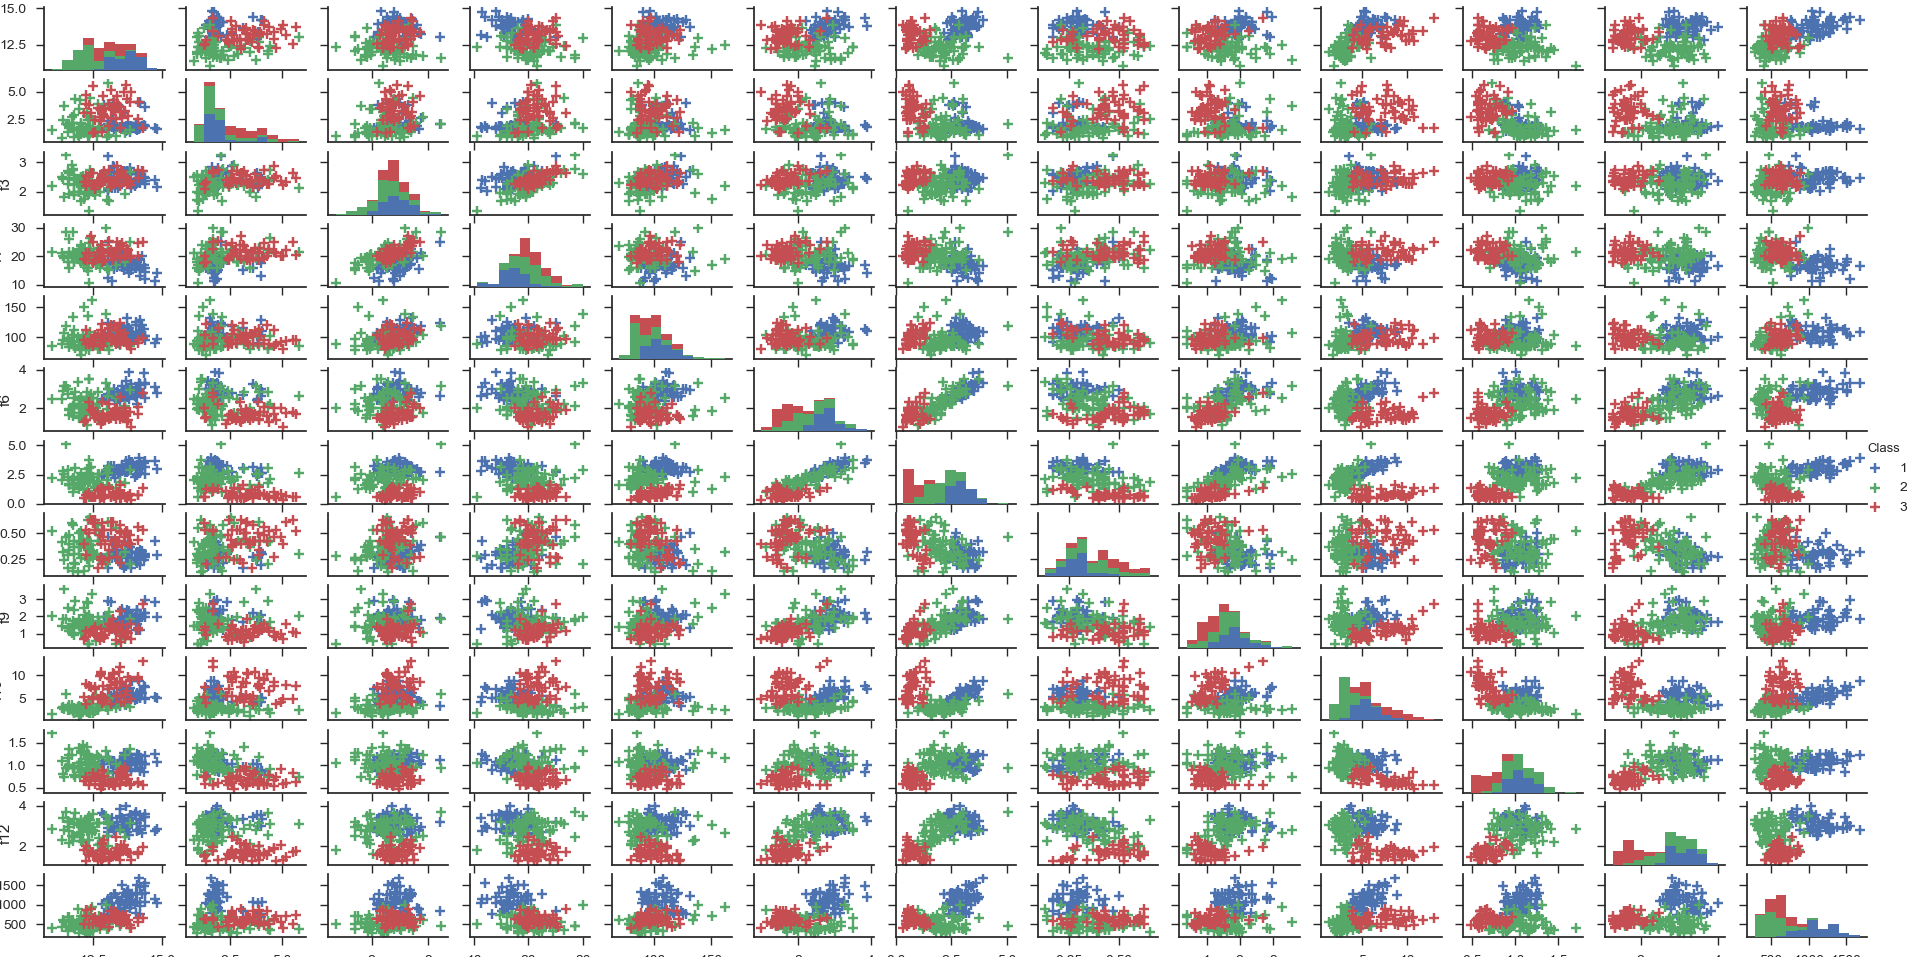
\includegraphics[width=1\textwidth]{dsWineCombined.png}
\caption{Rozkład cech dla zbioru Wine}
\end{figure}

\begin{figure}[H]
\centering
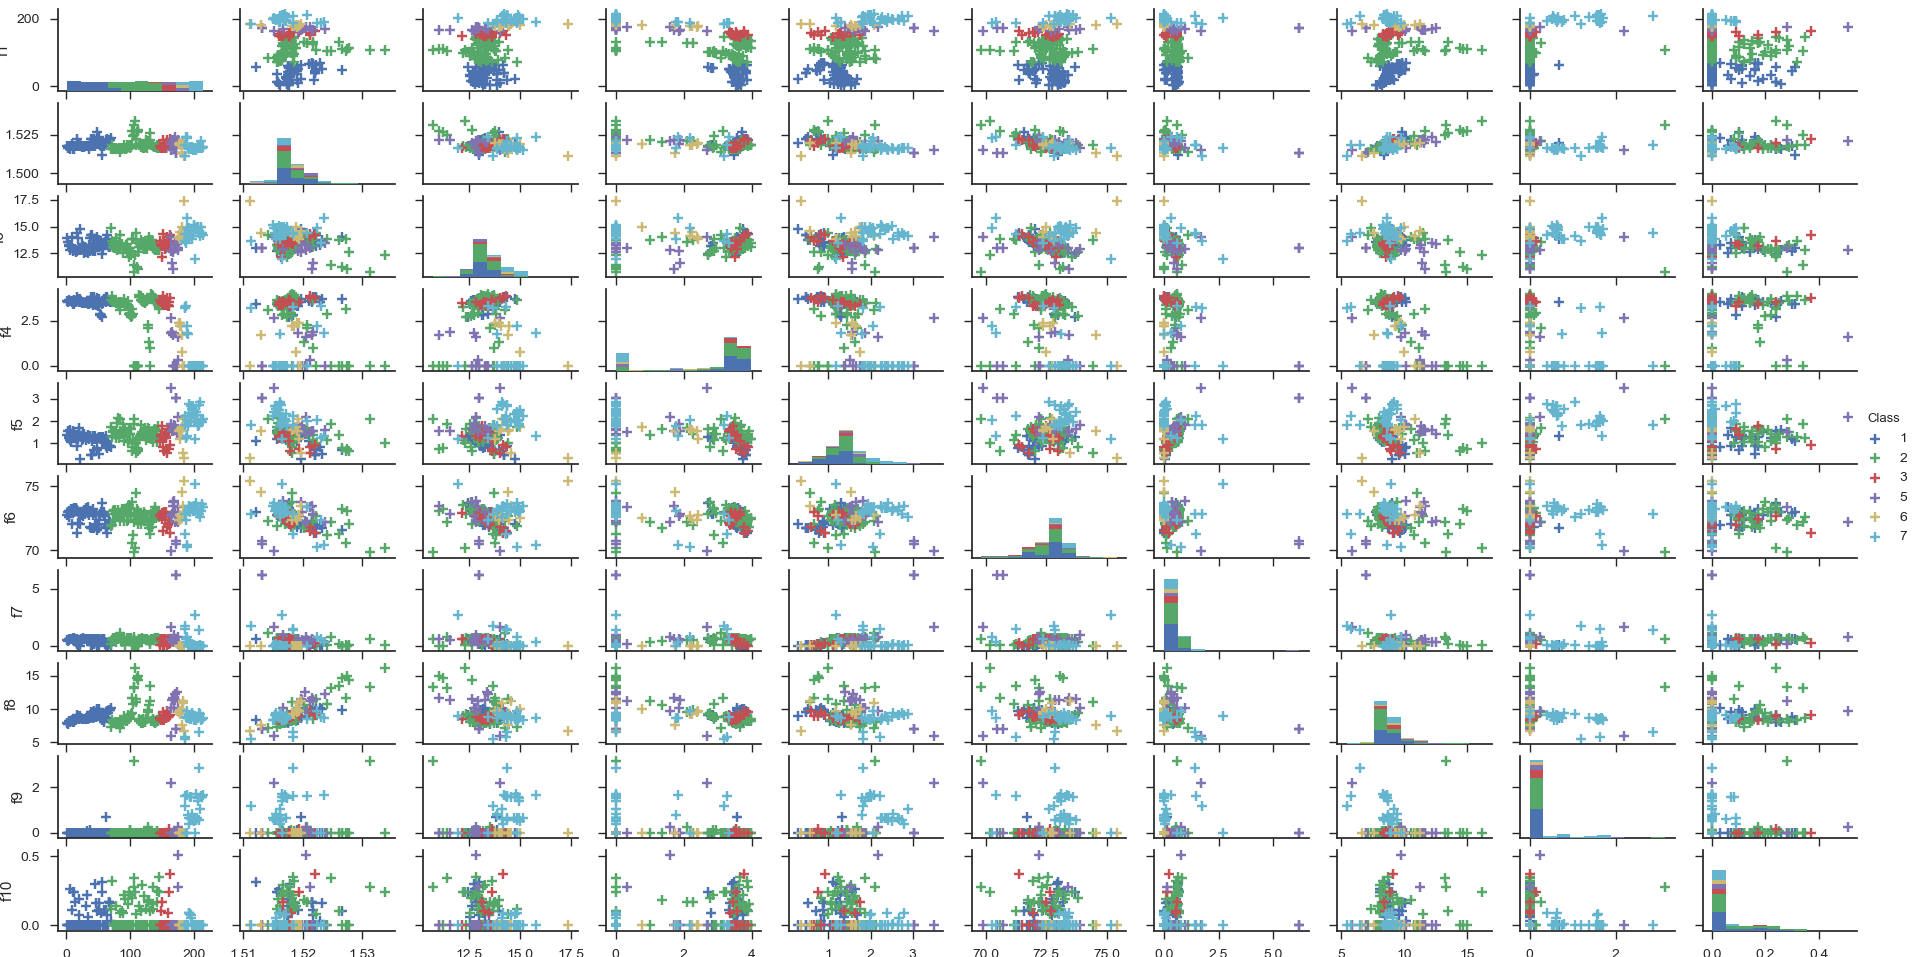
\includegraphics[width=1\textwidth]{dsGlassCombined.png}
\caption{Rozkład cech dla zbioru Glass}
\end{figure}

\begin{figure}[H]
\centering
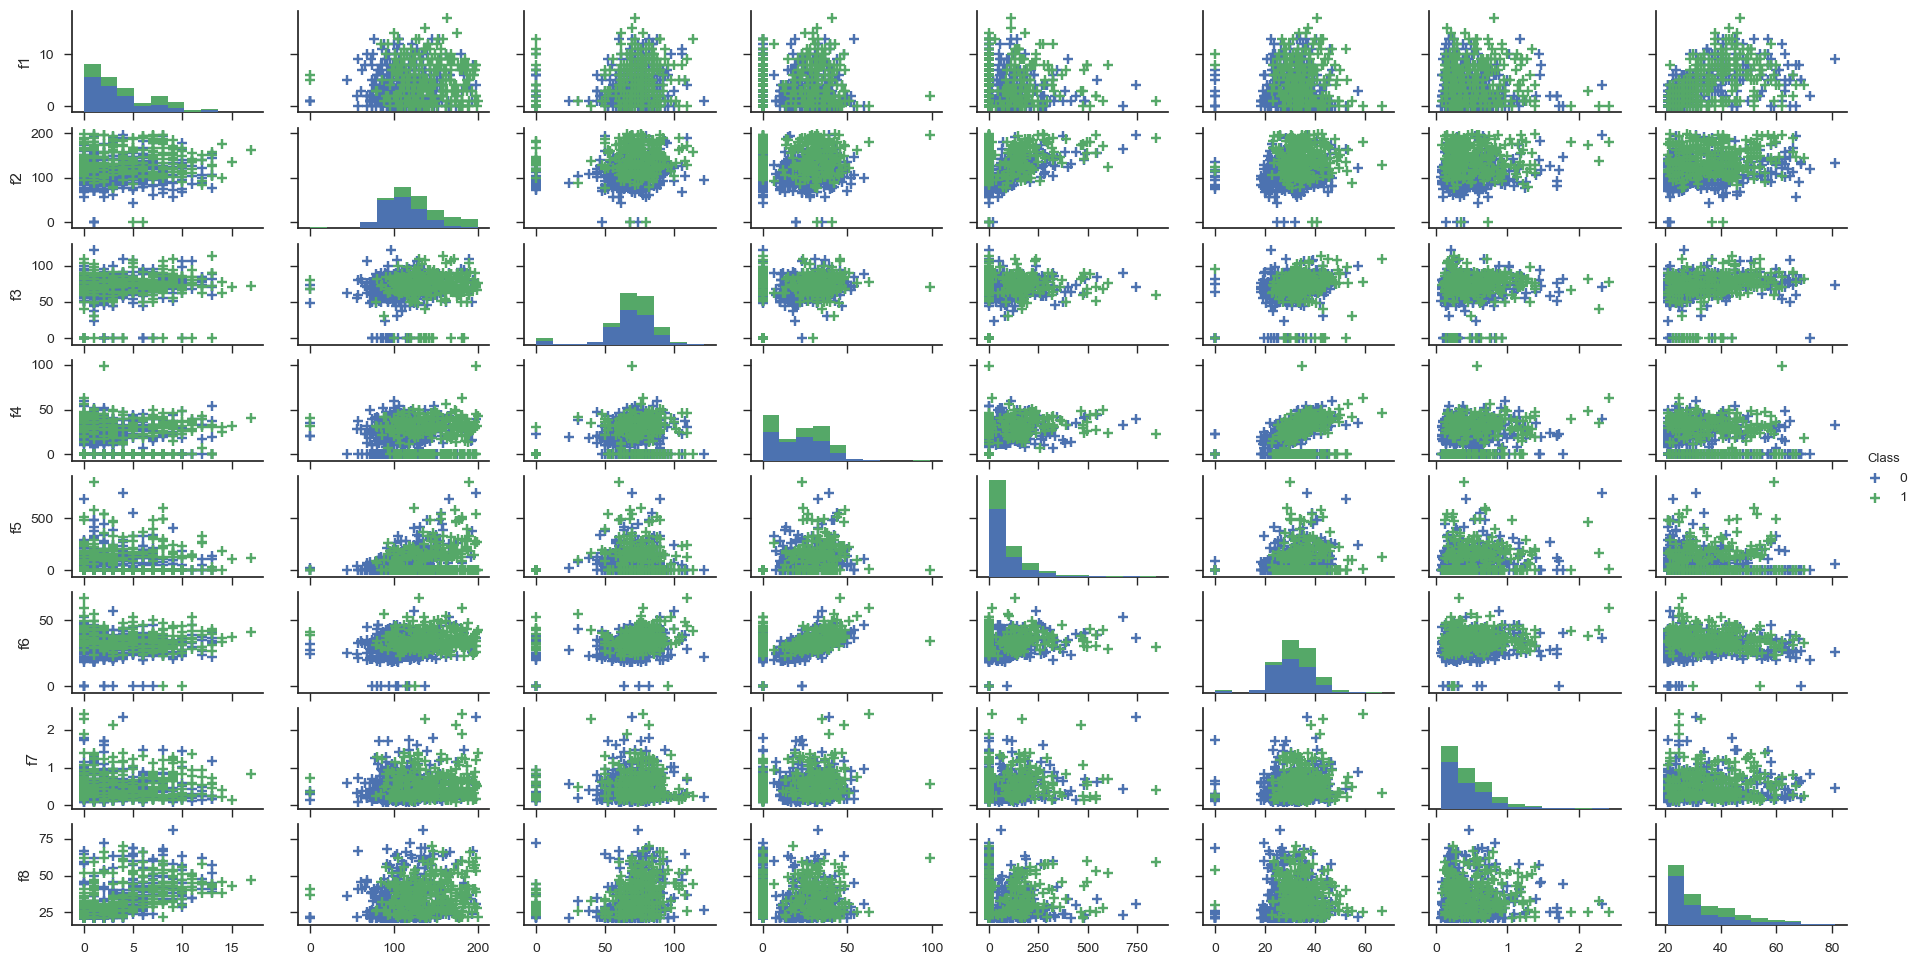
\includegraphics[width=1\textwidth]{dsDiabetesCombined.png}
\caption{Rozkład cech dla zbioru Diabetes}
\end{figure}

\section{Porównanie metod kroswalidacji}
Zaimplementowane zostały dwie metody kroswalidacji:
\\
\textsl{•} Niestratyfikowana (ręcznie)
\\
\textsl{•} Stratyfikowana (z pomocą biblioteki caret)
\\
Do porównania wyników użyty zostanie parametr fscore.

\begin{tabular}{ |p{2.3cm}||p{2.5cm}|p{3.5cm}|p{3.5cm}| }
 \hline
Folds&Stratified&Normall no randomize&Normall randomize\\
\hline
\multicolumn{4}{|c|}{WINE}\\
\hline
2 &0.8702254 &0.2159056 &0.8991312\\
3 &0.8813016 &0.179399 &0.9150061\\
4 &0.9326211 &0.6095417 &0.9105371\\
5 &0.9272085 &0.7563068 &0.9087973\\
6 &0.9437285 &0.8759431 &0.9097962\\
7 &0.9438199 &0.8265988 &0.9437564\\
8 &0.9380819 &0.904744 &0.938011\\
9 &0.9380761 &0.9104553 &0.9323077\\
10 &0.9154446 &0.8706026 &0.8985881\\
\hline
\multicolumn{4}{|c|}{GLASS}\\
\hline
2 &0.6392635 &0.1014686 &0.7088985\\
3 &0.6457611 &0.03486039 &0.701681\\
4 &0.675482 &0.2136425 &0.7084925\\
5 &0.6774104 &0.2178138 &0.659168\\
6 &0.7275745 &0.2381391 &0.6300857\\
7 &0.6519988 &0.2785823 &0.6405154\\
8 &0.6906709 &0.3186959 &0.6425939\\
9 &0.7124522 &0.2739046 &0.7037276\\
10 &0.6788223 &0.515942 &0.655208\\
\hline
\multicolumn{4}{|c|}{DIABETES}\\
\hline
2 &0.7654584 &0.8065448 &0.8108632\\
3 &0.7949952 &0.7971602 &0.8008256\\
4 &0.8078049 &0.8 &0.8079602\\
5 &0.7935549 &0.7980198 &0.781655\\
6 &0.8059406 &0.8036999 &0.8027478\\
7 &0.8023483 &0.8086359 &0.7988281\\
8 &0.7967644 &0.7976072 &0.8104449\\
9 &0.8251208 &0.810757 &0.8189739\\
10 &0.7935549 &0.8083416 &0.8050193\\
\hline
\end{tabular}
\vspace{5mm}
\vspace{5mm}





\section{Badane parametry}
Do zbadania wybrano wpływ modyfikacji 4 różnych parametrów na drzewo. Domyślna konfiguracja parametrów drzewa wygląda następująco:
(subset = TRUE, bands = 0, winnow = FALSE, noGlobalPruning = FALSE, CF = 0.25, minCases = 2, fuzzyThreshold = FALSE, sample = 0, seed = sample.int(4096, size = 1) -1L, earlyStopping = TRUE, label = "outcome")

MinCases - określa minimalną ilość próbek w danym liściu.

\begin{figure}[H]
\centering
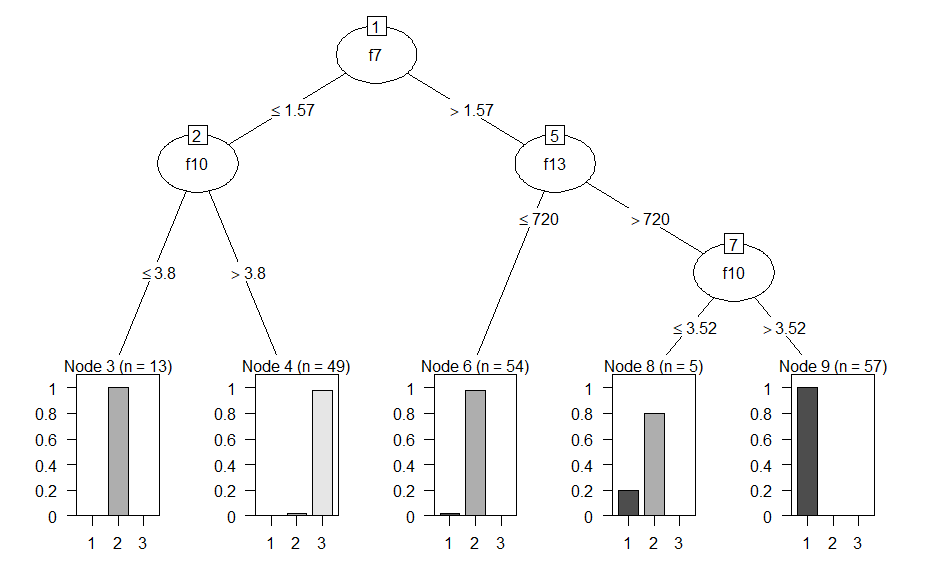
\includegraphics[width=1\textwidth]{wineMinCase5.png}
\caption{Drzewo klasyfikacji instancji wine przy ustawieniu parametru minCases = 5}
\end{figure}

\begin{figure}[H]
\centering
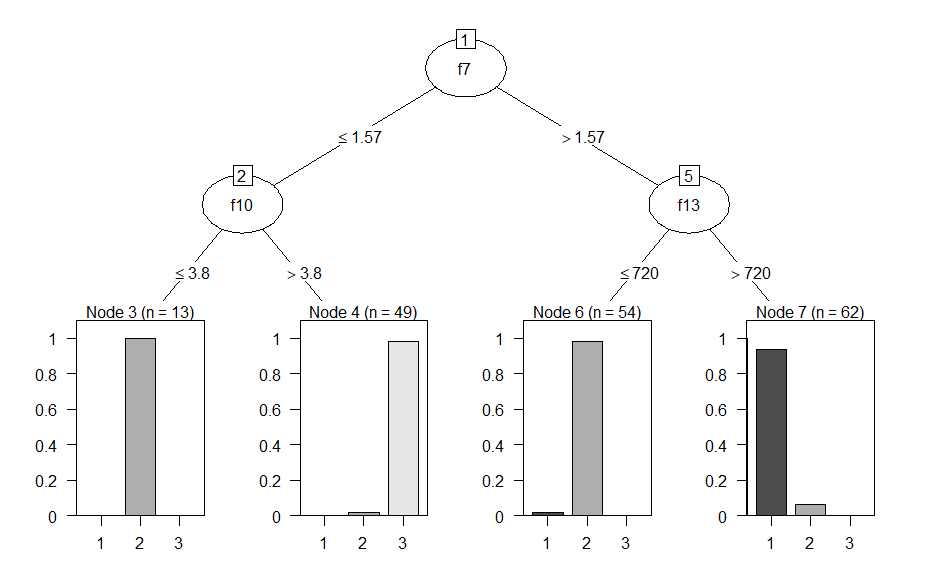
\includegraphics[width=1\textwidth]{wineMinCase10.png}
\caption{Drzewo klasyfikacji instancji wine przy ustawieniu parametru minCases = 10}
\end{figure}

\begin{figure}[H]
\centering
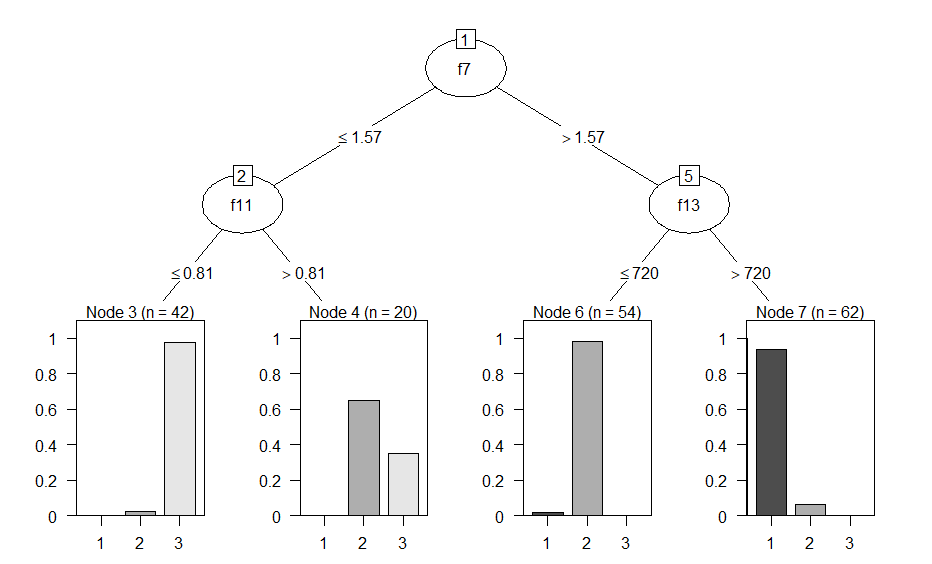
\includegraphics[width=1\textwidth]{wineMinCase20.png}
\caption{Drzewo klasyfikacji instancji wine przy ustawieniu parametru minCases = 20}
\end{figure}

CF - confidence factor - parametr przyjmujący wartość z zakresu od 0 do 1. Wraz ze zmniejszeniem wartości, zwiększy się ilość przycinanych węzłów. Pomaga zapobiegać zbyt dużemu rozrostowi drzewa, oraz zjawisku przeuczenia.

\begin{figure}[H]
\centering
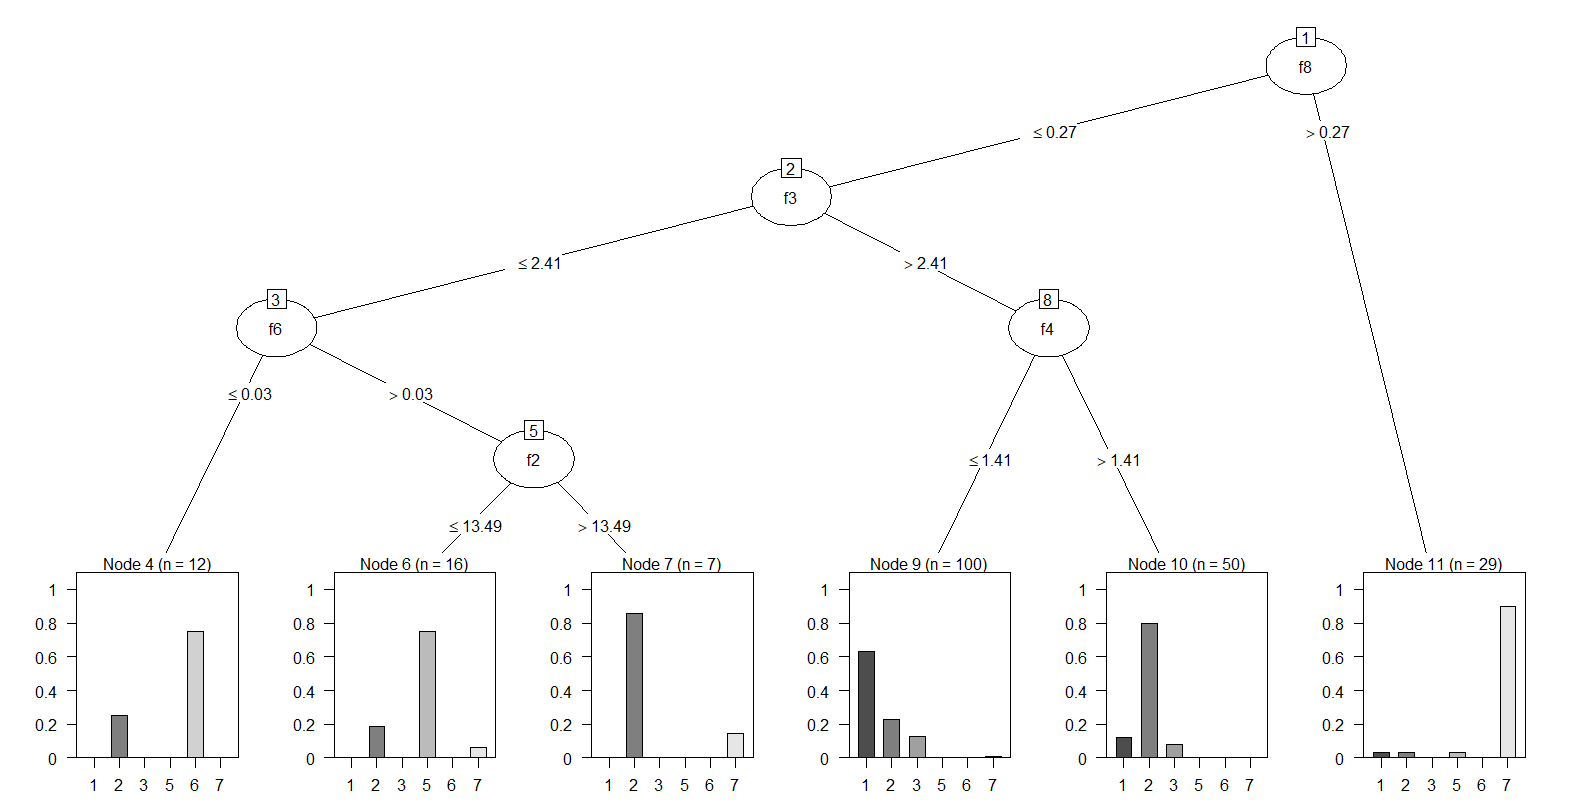
\includegraphics[width=1\textwidth]{glassCF_0.png}
\caption{Drzewo klasyfikacji instancji glass przy ustawieniu parametru CF = 0}
\end{figure}

\begin{figure}[H]
\centering
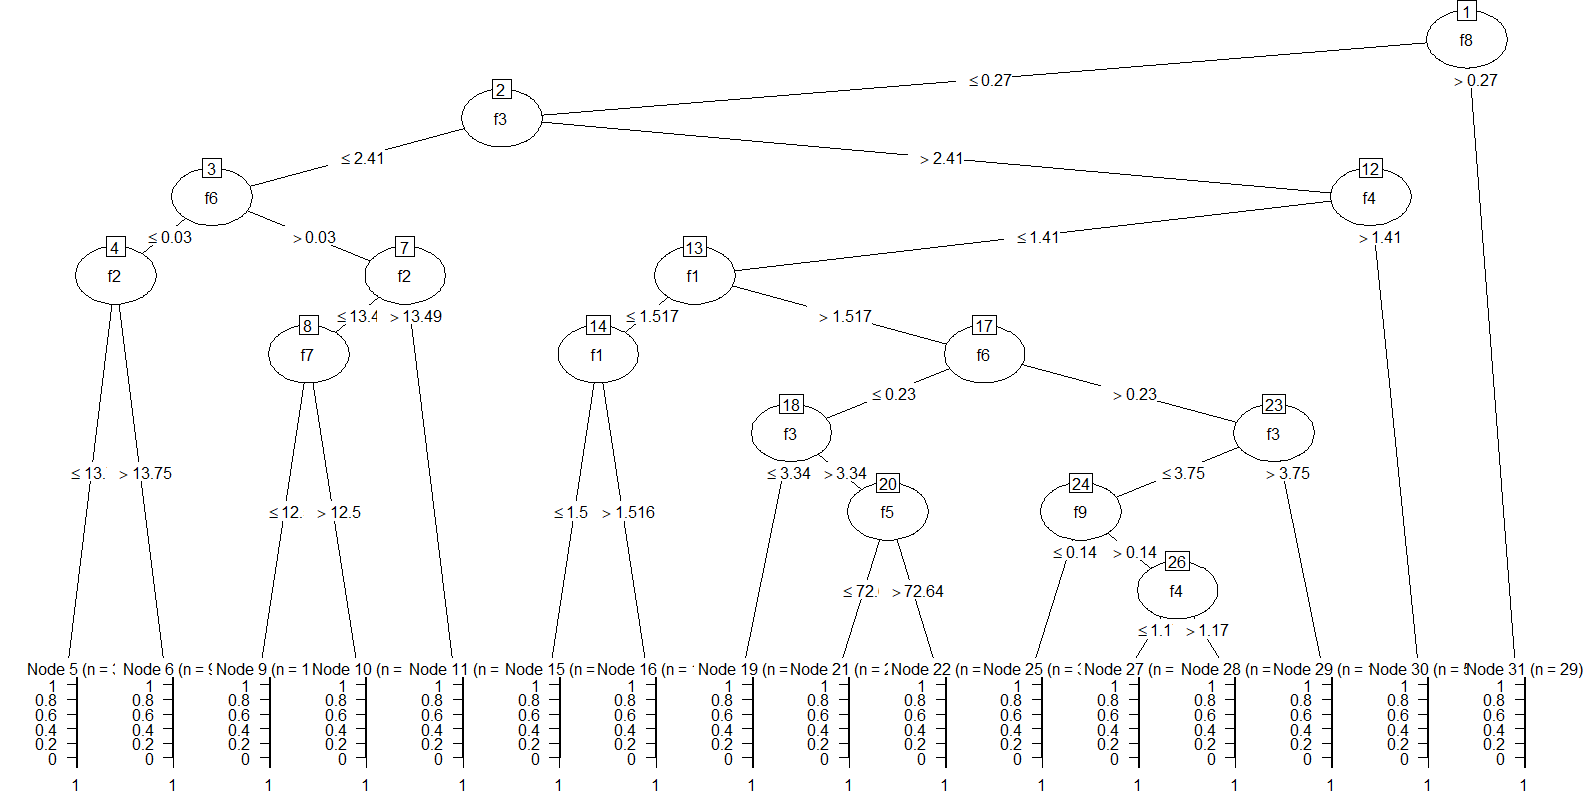
\includegraphics[width=1\textwidth]{glassCF_0_1.png}
\caption{Drzewo klasyfikacji instancji glass przy ustawieniu parametru CF = 0.1}
\end{figure}

\begin{figure}[H]
\centering
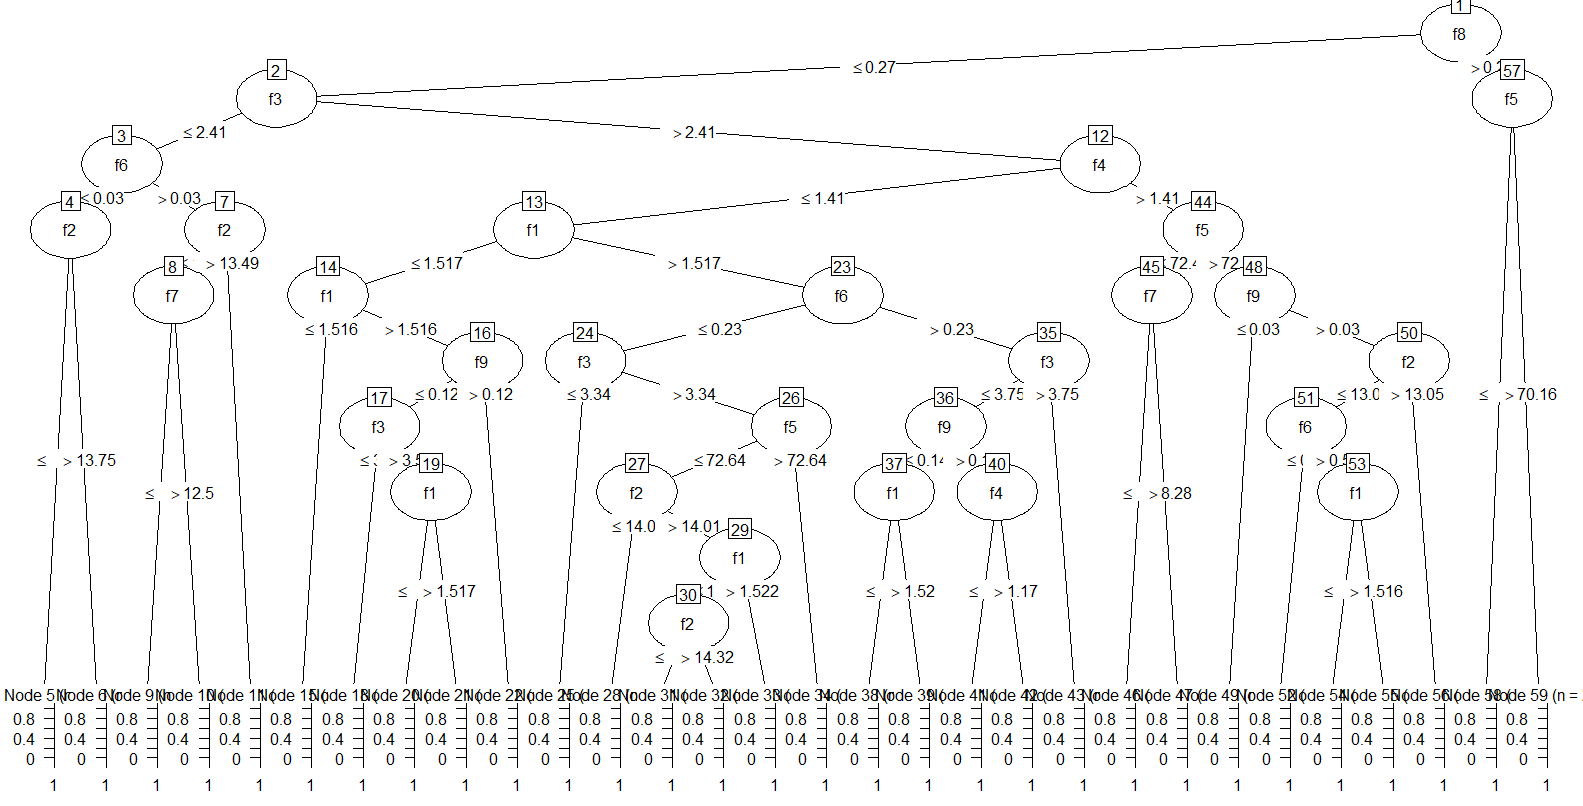
\includegraphics[width=1\textwidth]{glassCF_1.png}
\caption{Drzewo klasyfikacji instancji glass przy ustawieniu parametru CF = 1}
\end{figure}

noGlobalPruning - Przełącznik informujący czy powinien zostać wykonany końcowy krok odpowiedzialny za dodatkowe przycinanie drzewa w celu zmniejszenia jego rozmiaru.

\begin{figure}[H]
\centering
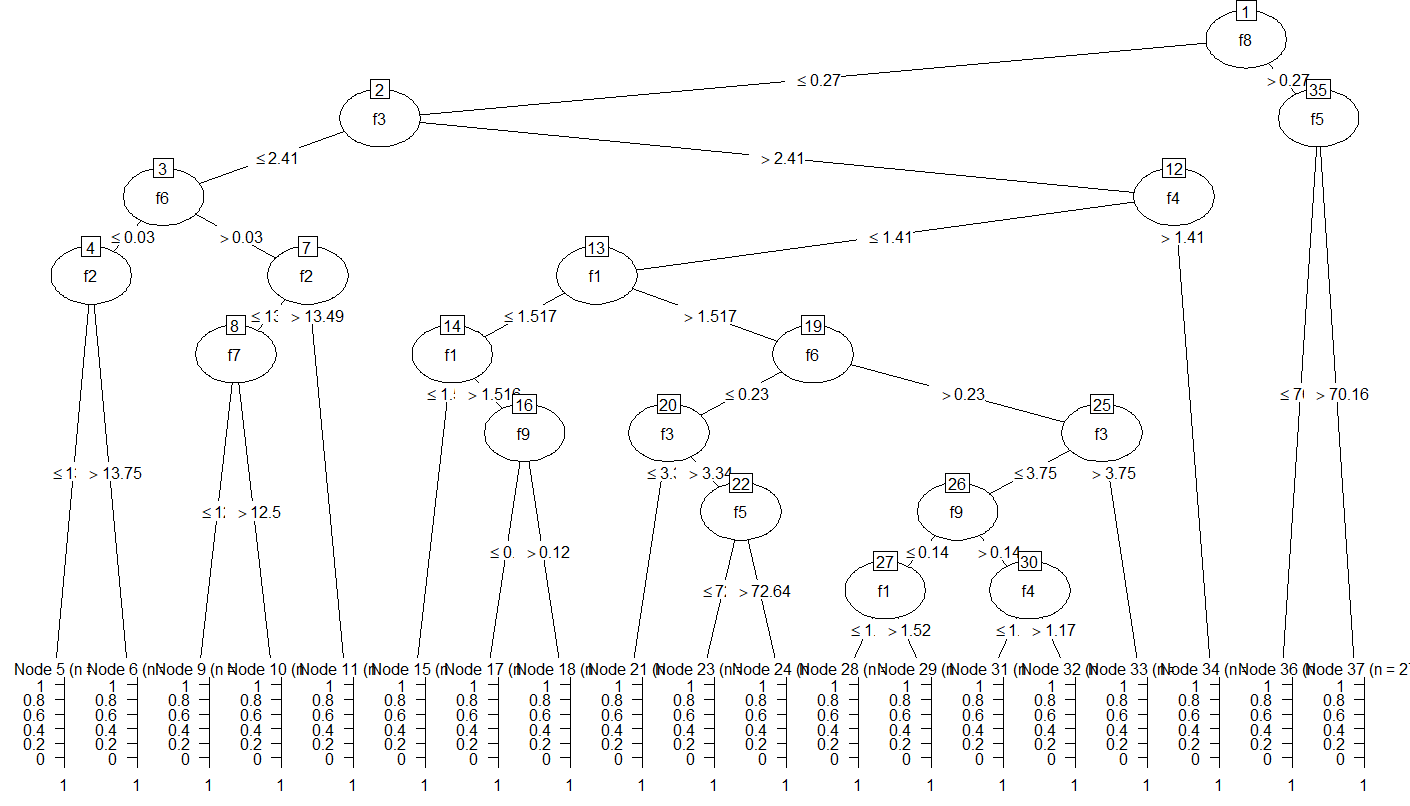
\includegraphics[width=1\textwidth]{no_GP_Glass.png}
\caption{Drzewo klasyfikacji instancji glass przy ustawieniu parametru noGlobalPruning = TRUE}
\end{figure}

\begin{figure}[H]
\centering
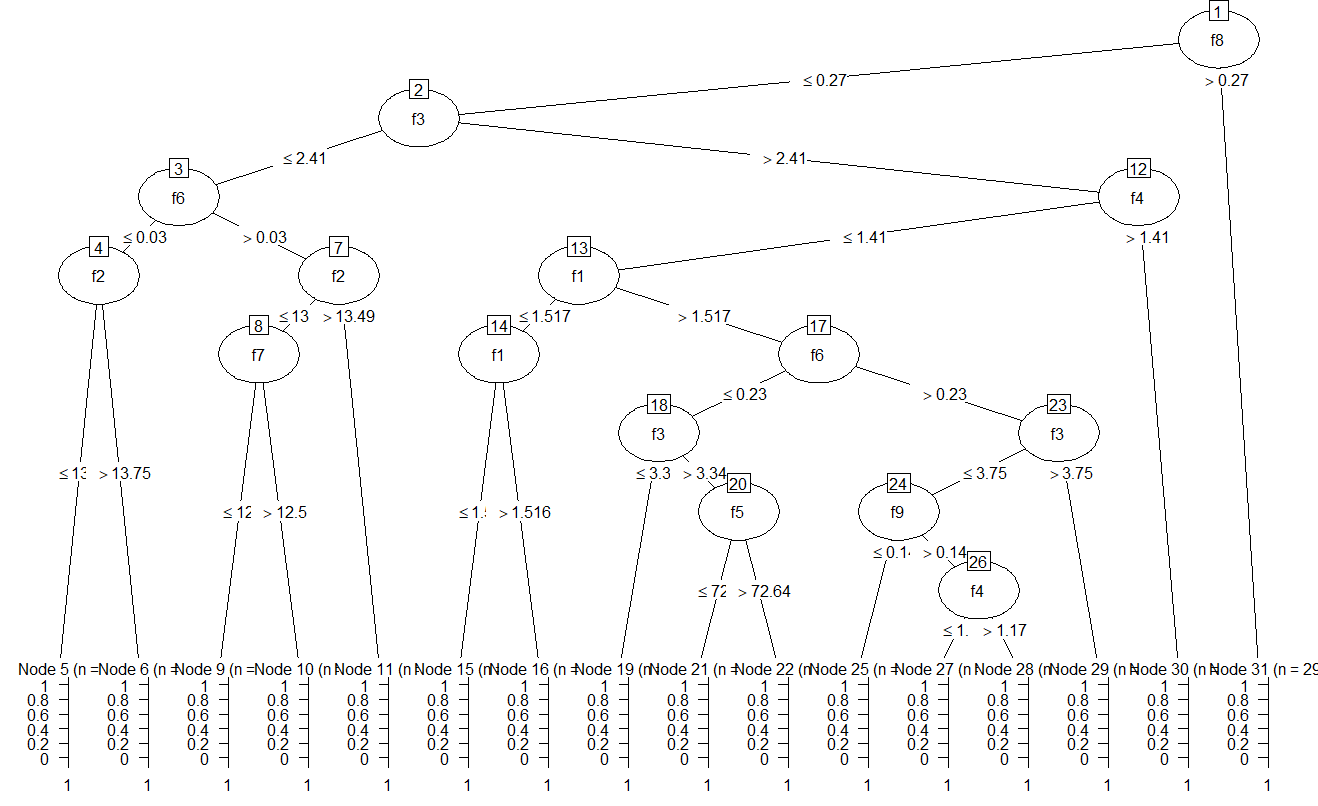
\includegraphics[width=1\textwidth]{GP_Glass.png}
\caption{Drzewo klasyfikacji instancji glass przy ustawieniu parametru noGlobalPruning = FALSE}
\end{figure}

winnowing - Czy powinien zostać zaaplikowany krok przesiewania. Polega on na wstępnej selekcji cech, które mają być wykorzystane do późniejszego modelowania drzewa. Dane zostają rozdzielone na dwie części i dopasowany zostaje inicjacyjny model. Każdy predyktor (przesłanka) jest kolejno eliminowana i sprawdzany jest wpływ takiej operacji na drzewo. Predyktory są oznaczane w zależności od tego czy wpływają one na zwiększenie ilości generowanych błędów.

\begin{figure}[H]
\centering
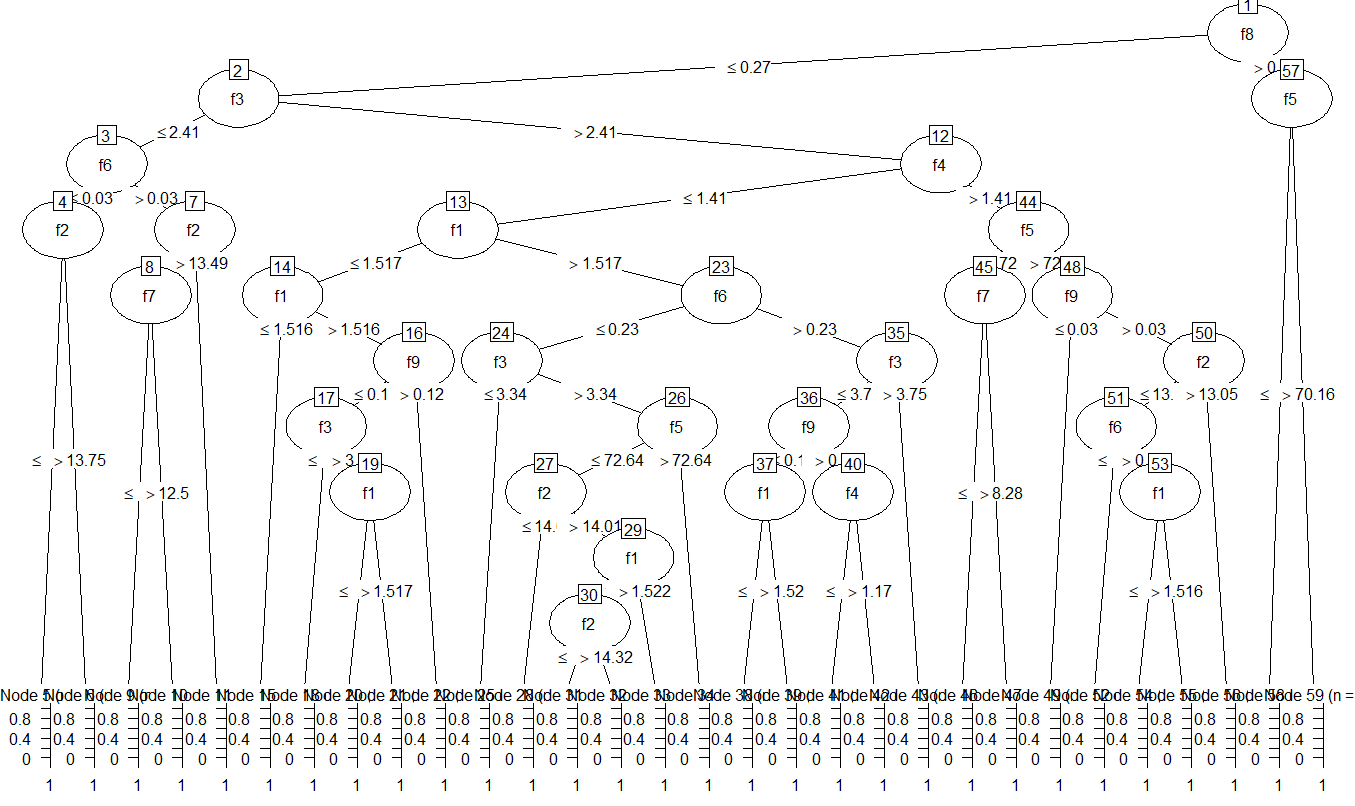
\includegraphics[width=1\textwidth]{glassWinnow_FALSE.png}
\caption{Drzewo klasyfikacji instancji glass przy ustawieniu parametru winnow = FALSE}
\end{figure}

\begin{figure}[H]
\centering
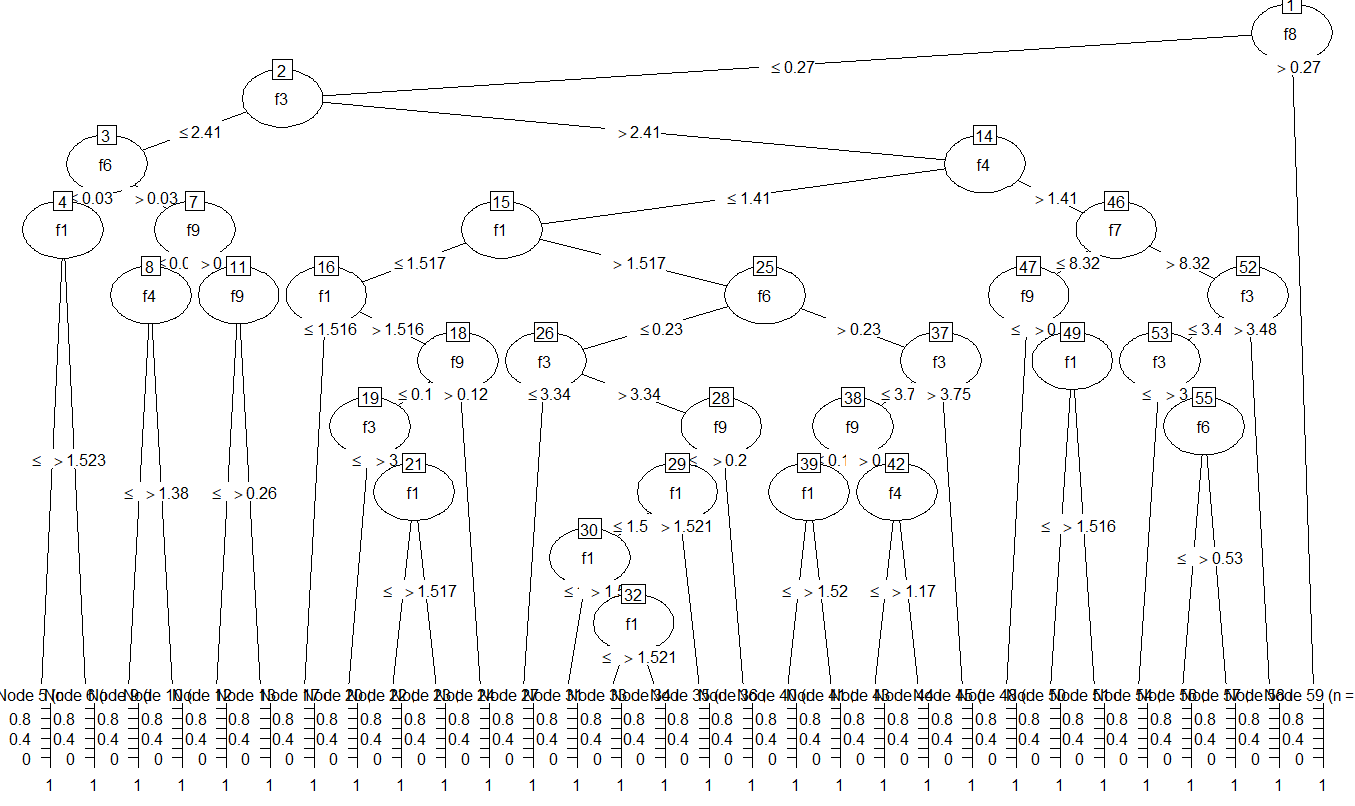
\includegraphics[width=1\textwidth]{glassWinnow_TRUE.png}
\caption{Drzewo klasyfikacji instancji glass przy ustawieniu parametru winnow = FALSE}
\end{figure}

\section{Wpływ parametrów na zbiór wine}

\begin{figure}[H]
\centering
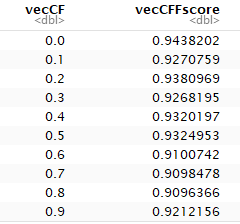
\includegraphics{wineDTCF.PNG}
\end{figure}

\begin{figure}[H]
\centering
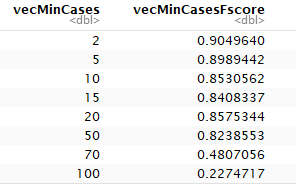
\includegraphics{wineDTminCases.png}
\end{figure}

\begin{figure}[H]
\centering
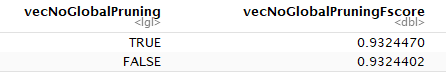
\includegraphics{wineDTnoGlobalPruning.PNG}
\end{figure}

\begin{figure}[H]
\centering
\includegraphics{WineDTwinnow.PNG}
\end{figure}

\begin{figure}[H]
\centering
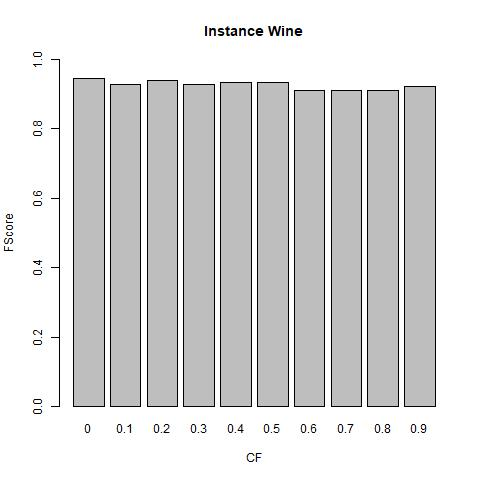
\includegraphics[width=0.7\textwidth]{WineFScoreCF.jpg}
\end{figure}

\begin{figure}[H]
\centering
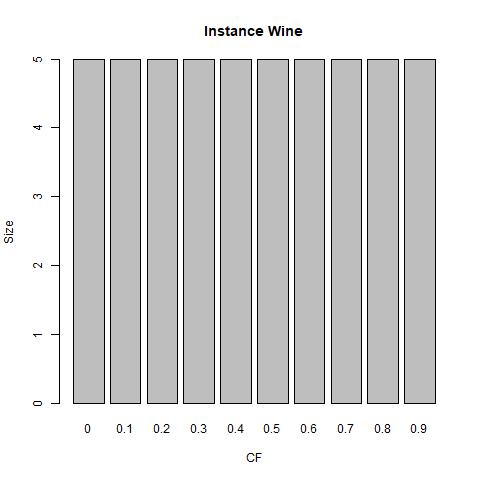
\includegraphics[width=0.7\textwidth]{WineSizeCF.jpg}
\end{figure}

\begin{figure}[H]
\centering
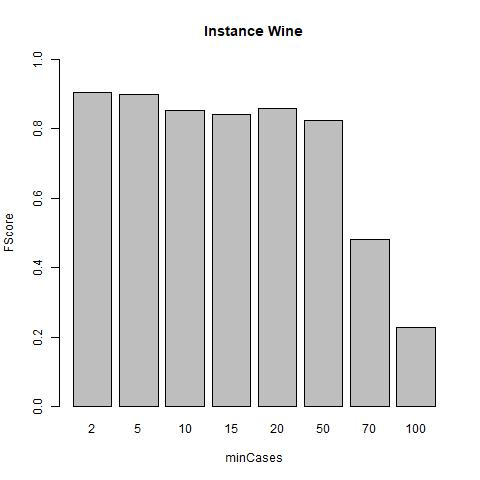
\includegraphics[width=0.7\textwidth]{WineFScoreMinCases.jpg}
\end{figure}

\begin{figure}[H]
\centering
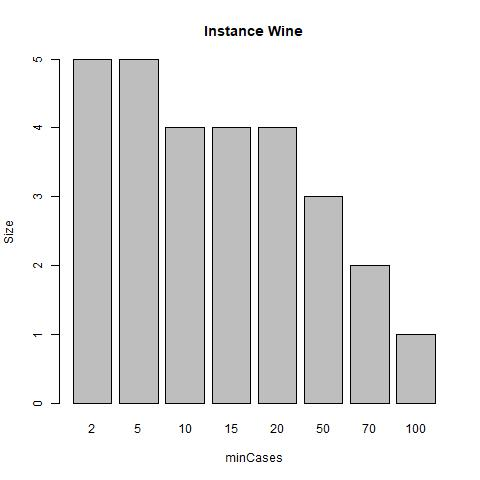
\includegraphics[width=0.7\textwidth]{WineSizeMinCases.jpg}
\end{figure}

\begin{figure}[H]
\centering
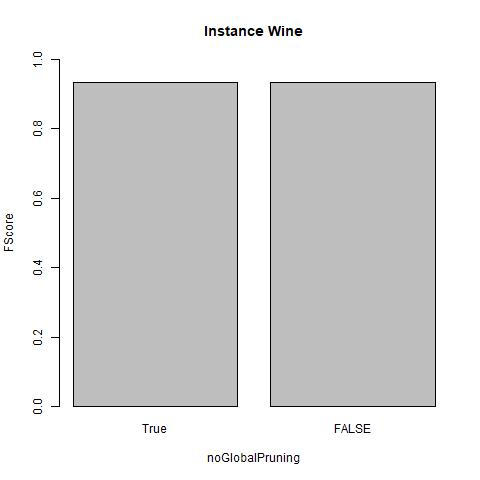
\includegraphics[width=0.7\textwidth]{WineFScoreNoGlobalPruning.jpg}
\end{figure}

\begin{figure}[H]
\centering
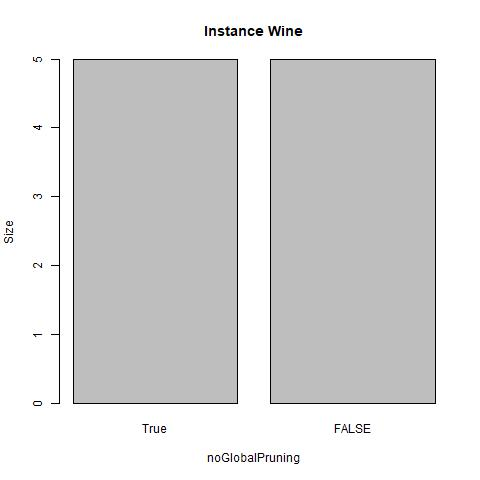
\includegraphics[width=0.7\textwidth]{WineSizeNoGlobalPruning.jpg}
\end{figure}

\begin{figure}[H]
\centering
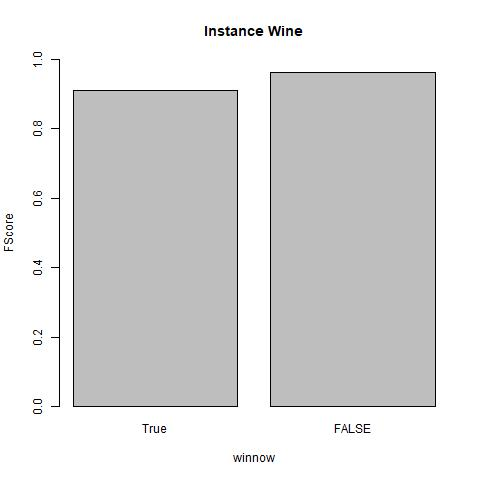
\includegraphics[width=0.7\textwidth]{WineFScoreWinnow.jpg}
\end{figure}

\begin{figure}[H]
\centering
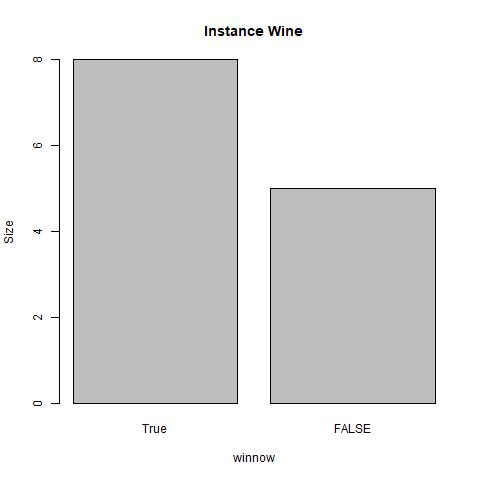
\includegraphics[width=0.7\textwidth]{WineSizeWinnow.jpg}
\end{figure}

\section{Wpływ parametrów na zbiór glass}

\begin{figure}[H]
\centering
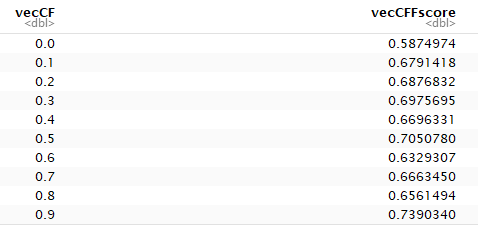
\includegraphics{glassDTCF.PNG}
\end{figure}

\begin{figure}[H]
\centering
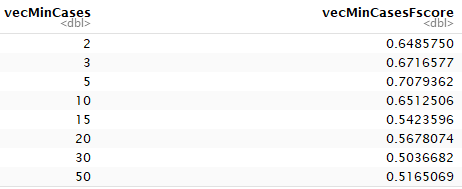
\includegraphics{glassDTminCases.png}
\end{figure}

\begin{figure}[H]
\centering
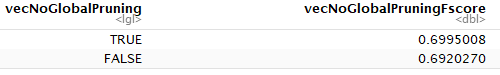
\includegraphics{glassDTnoGlobalPruning.PNG}
\end{figure}

\begin{figure}[H]
\centering
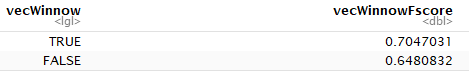
\includegraphics{glassDTwinnow.PNG}
\end{figure}

\begin{figure}[H]
\centering
\includegraphics[width=0.7\textwidth]{glassFScoreCF.jpg}
\end{figure}

\begin{figure}[H]
\centering
\includegraphics[width=0.7\textwidth]{glassSizeCF.jpg}
\end{figure}

\begin{figure}[H]
\centering
\includegraphics[width=0.7\textwidth]{glassFScoreMinCases.jpg}
\end{figure}

\begin{figure}[H]
\centering
\includegraphics[width=0.7\textwidth]{glassSizeMinCases.jpg}
\end{figure}

\begin{figure}[H]
\centering
\includegraphics[width=0.7\textwidth]{glassFScoreNoGlobalPruning.jpg}
\end{figure}

\begin{figure}[H]
\centering
\includegraphics[width=0.7\textwidth]{glassSizeNoGlobalPruning.jpg}
\end{figure}

\begin{figure}[H]
\centering
\includegraphics[width=0.7\textwidth]{glassFScoreWinnow.jpg}
\end{figure}

\begin{figure}[H]
\centering
\includegraphics[width=0.7\textwidth]{glassSizeWinnow.jpg}
\end{figure}

\section{Wpływ parametrów na zbiór diabetes}

\begin{figure}[H]
\centering
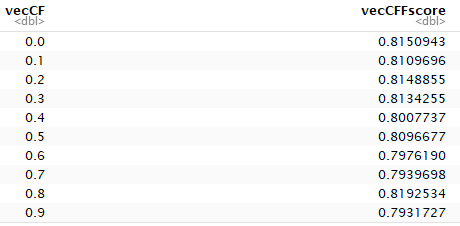
\includegraphics{diabetesDFCF.PNG}
\end{figure}

\begin{figure}[H]
\centering
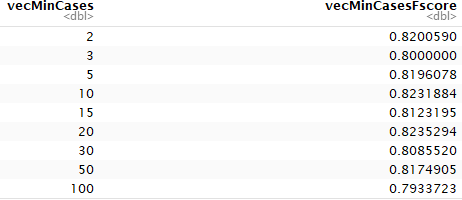
\includegraphics{diabetesDFminCases.png}
\end{figure}

\begin{figure}[H]
\centering
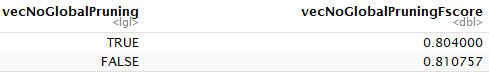
\includegraphics{diabetesDFnoGlobalPruning.PNG}
\end{figure}

\begin{figure}[H]
\centering
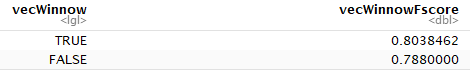
\includegraphics{diabetesDFwinnow.PNG}
\end{figure}

\begin{figure}[H]
\centering
\includegraphics[width=0.7\textwidth]{diabetesFScoreCF.jpg}
\end{figure}

\begin{figure}[H]
\centering
\includegraphics[width=0.7\textwidth]{diabetesSizeCF.jpg}
\end{figure}

\begin{figure}[H]
\centering
\includegraphics[width=0.7\textwidth]{diabetesFScoreMinCases.jpg}
\end{figure}

\begin{figure}[H]
\centering
\includegraphics[width=0.7\textwidth]{diabetesSizeMinCases.jpg}
\end{figure}

\begin{figure}[H]
\centering
\includegraphics[width=0.7\textwidth]{diabetesFScoreNoGlobalPruning.jpg}
\end{figure}

\begin{figure}[H]
\centering
\includegraphics[width=0.7\textwidth]{diabetesSizeNoGlobalPruning.jpg}
\end{figure}

\begin{figure}[H]
\centering
\includegraphics[width=0.7\textwidth]{diabetesFScoreWinnow.jpg}
\end{figure}

\begin{figure}[H]
\centering
\includegraphics[width=0.7\textwidth]{diabetesSizeWinnow.jpg}
\end{figure}



\section{Optymalne drzewa decyzyjne dla zbiorów danych}
Dla każdej instancji danych wybrany został zbiór parametrów, który powinien dążyć do polepszenia jakości klasyfikacji oraz minimalizacji drzewa, priorytezując jakość. Wyniki zostały przedstawione poniżej.

\vspace{5mm}
\begin{tabular}{ |p{3cm}||p{1cm}|p{2cm}|p{3cm}|p{2cm}|p{2cm}|}
\hline
Zbiór &CF &minCases &noGlobalPruning &winnow & F1\\
\hline
Wine &0 &5 &TRUE &FALSE &0.932\\
Glass &0.1 &5 &FALSE &TRUE &0.691\\
Diabetes &0.1 &20 &FALSE &FALSE &0.816\\
\hline
\end{tabular}
\vspace{5mm}

\begin{figure}[H]
\centering
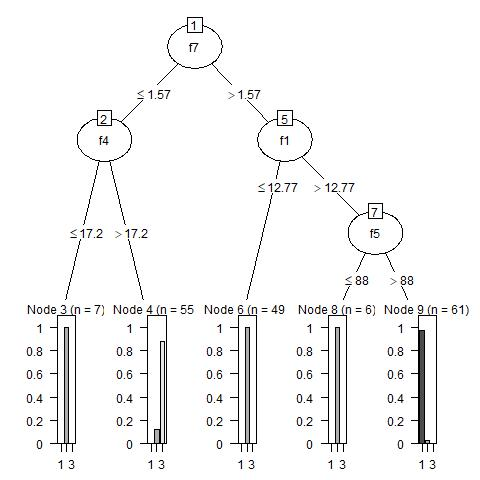
\includegraphics[width=1\textwidth]{wineOptimal.jpg}
\caption{Optymalne drzewo klasyfikujące dla instancji wine}
\end{figure}

\begin{figure}[H]
\centering
\includegraphics[width=1\textwidth]{glassOptimal.jpg}
\caption{Optymalne drzewo klasyfikujące dla instancji glass}
\end{figure}

\begin{figure}[H]
\centering
\includegraphics[width=1\textwidth]{diabetesOptimal.jpg}
\caption{Optymalne drzewo klasyfikujące dla instancji diabetes}
\end{figure}

\section{Porównanie wyników z metodą "Naive Bayes"}
Do porównania wyników między rezultatami otrzymanymi poprzez użycie drzewa decyzyjnego, a metodą "Naive Bayes" posłuży miara F1. Porównane zostaną najlepsze rezultaty.

\vspace{5mm}
\begin{tabular}{ |p{3cm}||p{3cm}|p{3cm}|}
\hline
Zbiór &C4.5 &Naive Bayes\\
\hline
Wine &0.932 &0.957\\
Glass &0.691 &0.646\\
Diabetes &0.816 &0.748\\
\hline
\end{tabular}
\vspace{5mm}

\begin{figure}[H]
\centering
\includegraphics[width=1\textwidth]{c4_5vsBayes.PNG}
\caption{Zestawienie wyników dla różnych klasyfikatorów}
\end{figure}

\section{Wnioski}
Zaimplementowane drzewa decyzyjne w przypadku dwóch zbiorów dały lepsze rezultaty. Dzięki odpowiedniej parametryzacji istnieje możliwość ograniczenia rozmiaru drzewa oraz polepszenia jakości klasyfikacji.//
Z powodu jasnych zasad klasyfikacji drzewa decyzyjne są przychylniej akceptowane przez specjalistów w wielu branżach niż deep learning, ponieważ łatwo można prześledzić każdą decyzję podejmowaną przez drzewo.//
Testy kroswalidacji po raz kolejny wykazały, że najlepszą metodą jest kroswalidacja stratyfikowana. Przed jej użyciem warto jednak zapoznać się z danymi wejściowymi, ponieważ w przypadku podziału na więcej foldów niż liczności najmniej licznej klasy wyniki mogą ulec pogorszeniu.

\end{document}